\section{Background}
\label{sec:background}

\subsection{Haskell}
\label{sec:haskell}

\newcommand{\CVar}{\texttt{Var}}
\newcommand{\CLit}{\texttt{Lit}}
\newcommand{\CApp}{\texttt{App}}
\newcommand{\CLam}{\texttt{Lam}}
\newcommand{\CLet}{\texttt{Let}}
\newcommand{\CCase}{\texttt{Case}}
\newcommand{\CType}{\texttt{Type}}
\newcommand{\CLocal}{\texttt{Local}}
\newcommand{\CGlobal}{\texttt{Global}}
\newcommand{\CLitNum}{\texttt{LitNum}}
\newcommand{\CLitStr}{\texttt{LitStr}}
\newcommand{\CDataAlt}{\texttt{DataAlt}}
\newcommand{\CLitAlt}{\texttt{LitAlt}}
\newcommand{\CDefault}{\texttt{Default}}
\newcommand{\CNonRec}{\texttt{NonRec}}
\newcommand{\CRec}{\texttt{Rec}}

\begin{figure}
  \begin{equation*}
    \begin{split}
      expr\    \rightarrow\ & \CVar\ id                                       \\
                         |\ & \CLit\ literal                                  \\
                         |\ & \CApp\ expr\ expr                               \\
                         |\ & \CLam\ \mathcal{L}\ expr                        \\
                         |\ & \CLet\ bind\ expr                               \\
                         |\ & \CCase\ expr\ \mathcal{L}\ \left[ alt \right]   \\
                         |\ & \CType                                          \\
      id\      \rightarrow\ & \CLocal\ \mathcal{L}                            \\
                         |\ & \CGlobal\ \mathcal{G}                           \\
      literal\ \rightarrow\ & \CLitNum\ \mathcal{N}                           \\
                         |\ & \CLitStr\ \mathcal{S}                           \\
      alt\     \rightarrow\ & ( altcon,\ [\mathcal{L}],\ expr )               \\
      altcon\  \rightarrow\ & \CDataAlt\ \mathcal{G}                          \\
                         |\ & \CLitAlt\ literal                               \\
                         |\ & \CDefault                                       \\
      bind\    \rightarrow\ & \CNonRec\ \mathcal{L}\ expr                     \\
                         |\ & \CRec\ [ ( \mathcal{L},\ expr ) ]
    \end{split}
  \end{equation*}
  Where:
  \begin{tabular}[t]{l @{ $=$ } l}
    $\mathcal{S}$ & string literals    \\
    $\mathcal{N}$ & numeric literals   \\
    $\mathcal{L}$ & local identifiers  \\
    $\mathcal{G}$ & global identifiers
  \end{tabular}

  \caption{Simplified syntax of GHC Core in BNF style. $[]$ and $(,)$ denote repetition and grouping, respectively.}
  \label{fig:coresyntax}
\end{figure}

We decided to focus on theory exploration in the Haskell programming language as it has mature, state-of-the-art implementations (\qspec{} \citep{QuickSpec} and \hspec{} \citep{claessen2013automating}). This is evident from the fact that the state-of-the-art equivalent for Isabelle/HOL, the \textsc{Hipster} \citep{Hipster} system, is actually implemented by translating to Haskell and invoking \hspec{}.

Haskell is well-suited to programming language research; indeed, this was a goal of the language's creators \citep{marlow2010haskell}. Like most members of the \emph{functional programming} paradigm, Haskell is essentially a variant of $\lambda$-calculus, with extra features such as a strong type system and ``syntactic sugar'' to improve readability. For simplicity, we will focus on an intermediate representation of the \textsc{GHC} compiler, known as \emph{GHC Core}, rather than the relatively large and complex syntax of Haskell proper. Core is based on \fc{}, but for our machine learning purposes we are mostly interested in its syntax; for a more thorough treatment of \fc{} and its use in GHC, see \citep[Appendix C]{sulzmann2007system}.

The sub-set of Core we consider is shown in figure \ref{fig:coresyntax}; compared to the full language \footnote{As of GHC version 7.10.2, the latest at the time of writing.} our major change is to ignore type hints (such as explicit casts, and differences between types/kinds/coercions). For brevity, we also omit several other forms of literal (machine words of various sizes, individual characters, etc.), as their treatment is similar to those of strings and numerals. We will use quoted strings to denote names and literals, e.g. \texttt{Local "foo"}, \texttt{Global "bar"}, \texttt{LitStr "baz"} and \texttt{LitNum "42"}, and require only that they can be compared for equality.

\begin{figure}
  \begin{haskell}
    data Nat = Z
             | S Nat

    plus :: Nat -> Nat -> Nat
    plus    Z  y = y
    plus (S x) y = S (plus x y)

    mult :: Nat -> Nat -> Nat
    mult    Z  y = Z
    mult (S x) y = plus y (mult x y)

    odd :: Nat -> Bool
    odd    Z  = False
    odd (S n) = even n

    even :: Nat -> Bool
    even    Z  = True
    even (S n) = odd n
  \end{haskell}
  \caption{A Haskell datatype for Peano numerals with some simple arithmetic functions, including mutually-recursive definitions for \hs{odd} and \hs{even}. \hs{Bool} is Haskell's built in boolean type, which can be regarded as \hs{data Bool = True \| False}.}
  \label{fig:haskellexample}
\end{figure}

\begin{figure}
  \begin{subfigure}[plus]{\textwidth}
    \begin{small}
      \underline{\texttt{plus}}
      \begin{verbatim}
Lam "a" (Lam "y" (Case (Var (Local "a"))
                       "b"
                       [(DataAlt "Z", [],    Var (Local "y")),
                        (DataAlt "S", ["x"], App (Var (Global "S"))
                                                 (App (App (Var (Global "plus"))
                                                           (Var (Local  "x")))
                                                      (Var (Local "y"))))]))
      \end{verbatim}
    \end{small}
  \end{subfigure}
  \begin{subfigure}[mult]{\textwidth}
    \begin{small}
      \underline{\texttt{mult}}
      \begin{verbatim}
Lam "a" (Lam "y" (Case (Var (Local "a"))
                       "b"
                       [(DataAlt "Z", [],    Var (Global "Z")),
                        (DataAlt "S", ["x"], App (App (Var (Global "plus"))
                                                      (Var (Local  "y")))
                                                 (App (App (Var (Global "mult"))
                                                           (Var (Local  "x")))
                                                      (Var (Local  "y"))))]))
      \end{verbatim}
    \end{small}
  \end{subfigure}
  \begin{subfigure}[odd]{\textwidth}
    \begin{small}
      \underline{\texttt{odd}}
      \begin{verbatim}
Lam "a" (Case (Var (Local "a"))
              "b"
              [(DataAlt "Z", [],    Var (Global "False")),
               (DataAlt "S", ["n"], App (Var (Global "even"))
                                        (Var (Local  "n")))])
      \end{verbatim}
    \end{small}
  \end{subfigure}
  \begin{subfigure}[even]{\textwidth}
    \begin{small}
      \underline{\texttt{even}}
      \begin{verbatim}
Lam "a" (Case (Var (Local "a"))
              "b"
              [(DataAlt "Z", [],    Var (Global "True")),
               (DataAlt "S", ["n"], App (Var (Global "odd"))
                                        (Var (Local  "n")))])
      \end{verbatim}
    \end{small}
  \end{subfigure}
  \caption{Translations of functions in figure \ref{fig:haskellexample} into the Core syntax of figure \ref{fig:coresyntax}. Notice the introduction of explicit $\lambda$ abstractions (\texttt{Lam}) and the use of \texttt{Case} to represent piecewise definitions. Fresh variables are chosen arbitrarily as \texttt{"a"}, \texttt{"b"}, etc.}
  \label{fig:coreexample}
\end{figure}

Figure \ref{fig:haskellexample} shows some simple Haskell function definitions, along with a custom datatype for Peano numerals. The translation to our Core syntax is routine, and shown in figure \ref{fig:coreexample}. Although the Core is more verbose, we can see that similar structure in the Haskell definitions gives rise to similar structure in the Core; for example, the definitions of \hs{odd} and \hs{even} are identical in both languages, except for the global variables. This correspondence allows us to analyse

Note that we exclude representations for type-level entities, including datatype definitions like that of \hs{Nat}. GHC can represent these, but in this work we only consider reducible expressions (i.e. value-level bindings of the form \hs{f a b ... = ...}).

\subsection{QuickCheck}
\label{sec:quickcheck}

Although unit testing is the de facto industry standard for quality assurance in non-critical systems, the level of confidence it provides is rather low, and totally inadequate for many (e.g. life-) critical systems. To see why, consider the following Haskell function, along with some unit tests:

\begin{lstlisting}[language=Haskell, xleftmargin=.2\textwidth, xrightmargin=.2\textwidth]
factorial 0 = 1
factorial n = n * factorial (n-1)

fact_base      = factorial 0 == factorial 1
fact_increases = factorial 3 <= factorial 4
fact_div       = factorial 4 == factorial 5 `div` 5
\end{lstlisting}

The intent of the function is to map an input $n$ to an output $n!$. The tests check a few properties of the implementation, including the base case, that the function is monotonically increasing, and a relationship between adjacent outputs. However, these tests will \emph{not} expose a serious problem with the implementation: it diverges on half of its possible inputs!

All of Haskell's built-in numeric types allow negative numbers, which this implementation doesn't take into account. Whilst this is a rather trivial example, it highlights a common problem: unit tests are insufficient to expose incorrect assumptions. In this case, our assumption that numbers are positive has caused a bug in the implementation \emph{and} limited the tests we've written.

If we do manage to spot this error, we might capture it in a \emph{regression test} and update the definition of \hs{factorial} to handle negative numbers, e.g. by taking their absolute value:

\iffalse TODO: Re-use these examples later on, e.g. for QuickSpec exploration \fi

\begin{lstlisting}[language=Haskell, xleftmargin=.2\textwidth, xrightmargin=.2\textwidth]
factorial 0 = 1
factorial n = let nPos = abs n
               in nPos * factorial (nPos - 1)

fact_neg = factorial 1 == factorial (-1)
\end{lstlisting}

However, this is \emph{still} not enough, since this function will also accept fractional values\footnote{Since we only use generic numeric operations, the function will be polymorphic with a type of the form \hs{forall t. Num t => t -> t}, where \hs{Num t} constrains the type variable \hs{t} to be numeric. In fact, Haskell will infer extra constraints such as \hs{Eq t} since we have used \hs{==} in the unit tests.}, which will also cause it to diverge. Clearly, by choosing what to test we are biasing the test suite towards those cases we've already taken into account, whilst neglecting the problems we did not expect.

Haskell offers a partial solution to this problem in the form of \emph{property checking}. Tools such as \qcheck{} separate tests into three components: a \emph{property} to check, which unlike a unit test may contain \emph{free variables}; a source of values to instantiate these free variables; and a stopping criterion. Here is how we might restate our unit tests as properties:

\begin{lstlisting}[language=Haskell, xleftmargin=.2\textwidth, xrightmargin=.2\textwidth]
fact_base        = factorial 0 == factorial 1
fact_increases n = factorial n <= factorial (n+1)
fact_div       n = factorial n == factorial (n+1) `div` (n+1)
fact_neg       n = factorial n == factorial (-n)
\end{lstlisting}

The free variables (all called \hs{n} in this case) are abstracted as function parameters; these parameters are implicitly \emph{universally quantified}, i.e. we've gone from a unit test asserting $factorial(3) \leq factorial(4)$ to a property asserting $\forall n, factorial(n) \leq factorial(n+1)$. Notice that unit tests like \hs{fact_base} are valid properties; they just assert rather weak statements.

To check these properties, \qcheck{} treats closed terms (like \hs{fact_base}) just like unit tests: pass if they evaluate to \hs{True}, fail otherwise. For open terms, a random selection of values are generated and passed in via the function parameter; the results are then treated in the same way as closed terms. The default stopping criterion for \qcheck{} (for each test) is when a single generated test fails, or when 100 generated tests pass.

The ability to state \emph{universal} properties in this way avoids some of the bias we encountered with unit tests. In the \hs{factorial} example, this manifests in two ways:

\begin{itemize}
  \item \qcheck{} cannot test polymorphic functions; they must be \emph{monomorphised} first (instantiated to a particular concrete type). This is a technical limitation, since \qcheck{} must know which type of values to generate, but in our example it would bring the issue with fractional values to our attention.

  \item The generators used by \qcheck{} depend only on the \emph{type} of value they are generating: since \hs{Int} includes positive and negative values, the \hs{Int} generator will output both. This will expose the problem with negative numbers, which we weren't expecting.
\end{itemize}

Property checking is certainly an improvement over unit testing, but the problem of tests being biased towards expected cases remains, since we are manually specifying the properties to be checked.

We can reduce this bias further through the use of \emph{theory exploration} tools, such as \qspec{} and \hspec{}. These programs \emph{discover} properties of a ``theory'' (e.g. a library), through a combination of brute-force enumeration, random testing and (in the case of \hspec{}) automated theorem proving.

\subsection{Theory Exploration}
\label{sec:theoryexploration}

In this work we consider the problem of \emph{(automated) theory exploration}, which includes the ability to \emph{generate} conjectures about code, to \emph{prove} those conjectures, and hence output \emph{novel} theorems without guidance from the user. The method of conjecture generation is a key characteristic of any theory exploration system, although all existing implementations rely on brute force enumeration to some degree.

We focus on \qspec{} \citep{QuickSpec}, which conjectures equations about Haskell code (these may be fed into another tool, such as \hspec{}, for proving). These conjectures are arrived at through the following stages:

\begin{enumerate}
  \item Given a typed signature $\Sigma$ and set of variables $V$, \qspec{} generates a list $terms$ containing the functions and constants from $\Sigma$, the variables from $V$ and type-correct function applications $f(x)$, where $f$ and $x$ are elements of $terms$. To ensure the list is finite, function applications are only nested up to a specified depth (by default, 3).
  \item The elements of $terms$ are grouped into equivalence classes, based on their type.
  \item Each variable is instantiated to a particular value, generated randomly by \qcheck{}.
  \item For each class, the members are compared (using a pre-specified function, such as equality \hs{==}) to see if these instantiations have caused an observable difference between members. If so, the class is split up to separate such distinguishable members.
  \item The previous steps of variable instantiation and comparison are repeated until the classes stabilise (i.e. no differences have been observed for some specified number of repetitions).
  \item A set of equations are then conjectured, relating each class's members.
\end{enumerate}

Such $conjectures$ can be used in several ways: they can be simplified for direct presentation to the user (by removing any equation which can be derived from the others by rewriting), sent to a more rigorous system like \hspec{} or \textsc{Hipster} for proving, or even serve as a background theory for an automated theorem prover \citep{claessen2013automating}.

As an example, we can consider a simple signature containing the expressions from figure \ref{fig:haskellexample}:

\begin{align*}
  \Sigma_{\texttt{Nat}} = \{\texttt{Z}, \texttt{S}, \texttt{plus}, \texttt{mult}, \texttt{odd}, \texttt{even}\}
\end{align*}

Together with a set of variables, say $V_{\texttt{Nat}} = \{a, b, c\}$, \qspec{}'s enumeration will resemble the following:

\begin{align*}
  terms_{\texttt{Nat}} = [& \texttt{Z},\ \texttt{S},\ \texttt{plus},\ \texttt{mult},\ \texttt{odd},\ \texttt{even},\ a,\ b,\ c,\ \texttt{S Z},\ \texttt{S}\ a,\ \texttt{S}\ b, \\
                     & \texttt{S}\ c,\ \texttt{plus Z},\ \texttt{plus}\ a,\ \dots ]
\end{align*}

Notice that Haskell curries functions, so the binary functions \hs{plus} and \hs{mult} can be treated as unary functions which return unary functions. This is required as the construction of $terms$ applies functions to one argument at a time.

\begin{figure}
  % To reproduce, run 'quickSpec nat' in haskell_example/src/QuickSpecExample.hs
  \begin{haskell}
                  plus a b = plus b a
                  plus a Z = a
         plus a (plus b c) = plus b (plus a c)
                  mult a b = mult b a
                  mult a Z = Z
         mult a (mult b c) = mult b (mult a c)
              plus a (S b) = S (plus a b)
              mult a (S b) = plus a (mult a b)
         mult a (plus b b) = mult b (plus a a)
                 odd (S a) = even a
            odd (plus a a) = odd Z
           odd (times a a) = odd a
                even (S a) = odd a
           even (plus a a) = even Z
          even (times a a) = even a
plus (mult a b) (mult a c) = mult a (plus b c)
  \end{haskell}
  \caption{Equations conjectured by \qspec{} for the functions in figure \ref{fig:haskellexample}; after simplification.}
  \label{fig:qspecresult}
\end{figure}

These terms will be grouped into five classes, one each for \hs{Nat}, \hs{Nat -> Nat} and \hs{Nat -> Nat -> Nat}, \hs{Nat -> Bool} and \hs{Bool}. As the variables $a$, $b$ and $c$ are instantiated to various randomly-generated numbers, these equivalence classes will be divided, until eventually the equations in figure \ref{fig:qspecresult} are conjectured.

Although complete, this enumeration approach is wasteful: many terms are unlikely to appear in theorems, which requires careful choice by the user of what to include in the signature. Here we know that addition and multiplication are closely related, and hence obey many algebraic laws. Our machine learning technique aims to predict these kinds of relations between functions, so we can create small signatures which nevertheless have the potential to give rise to many equations.

\qspec{} (and \hspec{}) is also compatible with Haskell's existing testing infrastructure, such that an invocation of \texttt{cabal test} can run these tools alongside more traditional QA tools like \qcheck{}, \textsc{HUnit} and \textsc{Criterion}.

In fact, there are similarities between the way a TE system like \qspec{} can generalise from checking \emph{particular} properties to \emph{inventing} new ones, and the way counterexample finders like \qcheck{} can generalise from testing \emph{particular} expressions to \emph{inventing} expressions to test. One of our aims is to understand the implications of this generalisation, the lessons that each can learn from the other's approach to term generation, and the consequences for testing and QA in general.

\subsection{Clustering}
\label{sec:clustering}

Our approach to scaling up these Haskell theory exploration tools takes inspiration from two sources. The first is premise selection, which makes expensive algorithms used in theorem proving more practical by limiting the size of their inputs. We describe this approach in more details in \S \ref{sec:relevance}. Premise selection is a practical tool which has existing applications in software, such as the \emph{Sledgehammer} component of the Isabelle/HOL theorem prover.

Despite the idea's promise, we cannot simply invoke existing premise selection algorithms in our theory exploration setting. The reason is that premise selection requires a distinguished expression to compare everything against; in practice this is the current goal of a theorem prover. Theory exploration does not have such a distinguished expression; instead, we are interested in relationships between \emph{any} terms generated from a signature, and hence we must consider the relevance of \emph{all terms} to \emph{all other terms}.

A natural fit for this task is \emph{clustering}, which attempts to group similar inputs together in an unsupervised way. Based on their success in discovering relationships and patterns between expressions in Coq and ACL2 (in the ML4PG and ACL2(ml) tools respectively), we hypothesise that clustering methods can fulfil the role of relevance filters for theory exploration: intelligently breaking up large signatures into smaller ones more amenable to brute force enumeration, such that related expressions are explored together.

\subsubsection{Feature Extraction}
\label{sec:featureextraction}

Before describing clustering in detail, we must introduce the idea of \emph{feature extraction}. This is the conversion of ``raw'' input data, such as audio, images or (in our case) Core expressions, into a form more suited to machine learning algorithms. By pre-processing our data in this way, we can re-use the same ``off-the-shelf'' machine learning algorithms in a variety of domains.

We use a standard representation of features as a \emph{feature vector} of numbers $(x_1, \dots, x_p)$ where $x_i \in \mathbb{R}$. \footnote{In fact, we only use $\mathbb{R}$ for notational and analytic convenience. Practical implementations will use an approximate format such as IEEE 754 floating point numbers.} For learning purposes this has two important advantages over our raw expressions:

\begin{itemize}
  \item All of our feature vectors will be the same size, i.e. they will all have length (or \emph{dimension}) $p$. This makes element-wise comparison between arbitrary feature vectors $\mathbf{x}$ and $\mathbf{y}$ trivial: compare each element $x_i$ with $y_i$ for $1 \leq i \leq p$. For expressions would not be so straightforward, as their nesting may give rise to very different shapes.
  \item Unlike our expressions, which are discrete, we can continuously transform one feature vector into another. This enables many powerful ML algorithms to be used, such as those based on \emph{gradient descent} or, in our case, arithmetic means.
\end{itemize}

\subsubsection{K-Means}
\label{sec:kmeans}

Clustering is an unsupervised machine learning task for grouping $n$ data points using a similarity metric. There are many variations on this theme, but in our case we make the following choices:

\begin{itemize}
  \item We fix the number of clusters at $k = \lceil \sqrt{n} \rceil$.
  \item Data points will be $p$-dimensional feature vectors, as defined above.
  \item We will use euclidean distance (denoted $d$) as our similarity metric.
  \item Clustering will be performed by the $k-means$ algorithm.
\end{itemize}

This is a standard setup, supported by off-the-shelf tools. In particular, it is similar to that used by the ML4PG and ACL2(ml) systems which served as inspiration for this work, which makes our results more easily comparable.

The k-means algorithm works, as the name suggests, by calculating the \emph{mean value} of each cluster's elements. Since k-means is iterative, we will use function notation to denote time steps, so $x(t)$ denotes the value of $x$ at time $t$. We denote the clusters as $C^1$ to $C^k$, their mean values as $\mathbf{m}^1$ to $\mathbf{m}^k$. Subscripts are vector elements, so $m^i_j(t)$ is the $i$th element of the $j$th mean, at time $t$.

Before k-means starts, we must choose \emph{seed} values for $\mathbf{m}^1(0)$ to $\mathbf{m}^k(0)$. Many methods have been proposed for choosing these values, e.g. see \citep{arthur2007k}. For simplicity, we will assume they are chosen at random from our data set. Subsequent values, i.e. $\mathbf{m}^i(t)$ for $t > 0$, are simply the mean values of the corresponding cluster $C^i(t)$:

\begin{equation}
  m^i_j(t) = \frac{\sum_{x \in C^i(t)} x_j}{|C^i(t)|}
\end{equation}

At time step $t$, the elements of each cluster $C_i^t$ are the data points closest to $m_i^{t-1}$ from the previous time step:

\begin{equation}
  C_i^t = \{ p \in S \mid i = \argmin\limits_j d(p, m_j^{t-1}) \}
\end{equation}

The mean values o determine which cluster a point $p$ belongs to, we
The as the name suggests, relies on the mean value of each cluster to determine  represents each cluster by uses a \emph{representative} t step $t$, the with cluster membership  We begin at iteration 0 by \emph{seeding} the algorithm with , each cluster is represented by the mean value of its elements:

\begin{equation}
  C_k =
\end{equation}



Both of these approaches, premise selection and clustering, use \emph{machine learning} (ML) algorithms to analyse expressions, and hence rely on \emph{feature extraction} to transform the data into a suitable representation and remove irrelevant details. This has two benefits:

\begin{itemize}
  \item \emph{Feature vectors} (ordered lists of features) are chosen to represent the relevant information in a more compressed form than the raw data (for example, replacing descriptive identifier names with sequential numbers). This reduces the input size of the machine learning problem, improving efficiency (e.g. running time).
  \item We avoid learning irrelevant details, such as the text encoding system used, improving \emph{data} efficiency (the number of samples required to spot a pattern).
\end{itemize}

Another benefit of feature extraction is to \emph{normalise} the input data to a fixed-size representation. Many ML algorithms only work with inputs of a uniform size; feature extraction allows us to use these algorithms in domains where the size of each input is not known, may vary or may even be unbounded.

In our case, we will use a novel feature extraction algorithm, described in \S \ref{sec:recurrentclustering}, to transform expressions in Haskell Core into a fixed size representation, suitable for clustering via the standard \emph{k-means} algorithm.

\iffalse TODO: I have had a look now at section 5. I do not think feature extraction and clustering is explained/defined there, either. Seeing your contribution is feature extraction algorithms, you need to define feature vectors and clusters *here* \fi

\begin{figure}
  \centering
  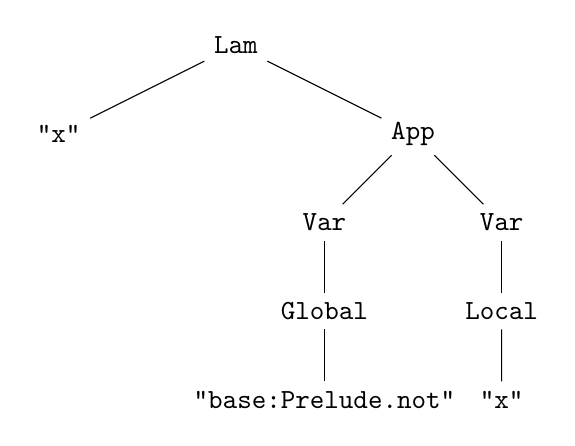
\begin{tikzpicture}[scale=0.75, level/.style={sibling distance=60mm/#1}]
      % Tree
      \node {\texttt{Lam}}
        child {node {\texttt{"x"}}}
        child {node {\texttt{App}}
          child {node {\texttt{Var}}
            child {node {\texttt{Global}}
              child {node {\texttt{"base:Prelude.not"}}}}}
          child {node {\texttt{Var}}
            child {node {\texttt{Local}}
              child {node {\texttt{"x"}}}}}};

      % Arrow
      %\node[single arrow,
      %      draw=black,
      %      fill=black!10,
      %      minimum height=2cm,
      %      shape border rotate=0] at (0,-1) {};
      %\draw[-latex] (A.east) -- (B.west);

      % Feature vector

  \end{tikzpicture}

  \caption{}

  \label{fig:featureextractionpic}
\end{figure}
